\section{Contract Language}
\label{sec:lang}

\begin{figure}
\begin{smathpar}
\renewcommand{\arraystretch}{1.2}
\begin{array}{rclcl}
\multicolumn{5}{c}{
  {x,y,\cureff} \in \mathtt{EffVar} \qquad \qquad
  {\sf Op} \in \mathtt{OperName}
}\\
\cv 		& \in & \mathtt{Contract} 	& \coloneqq & \forall (x : \tau).\cv
        \ALT \forall x.\cv \ALT \pi \\
\tau		& \in	& \mathtt{EffType}	& \coloneqq &  {\sf Op}
        \ALT \tau \vee \tau \\
\pi			&	\in & \mathtt{Prop} & \coloneqq & \true \ALT R(x,y)
        \ALT \pi \vee \pi \\
			  & 		&	 &  \ALT & \pi \wedge \pi \ALT \pi \Rightarrow \pi \\
R				& \in & \mathtt{Relation}	& \coloneqq & \visZ \ALT \soZ
        \ALT \sameobjZ \ALT = \\
				&			&	 &  \ALT & R \cup R \ALT R \cap R \ALT R^+ \\
\end{array}
\end{smathpar}
\caption{Contract language.}
\label{fig:contract-lang}
\end{figure}


\subsection{Syntax}

The syntax of our core contract language is shown in Figure
~\ref{fig:contract-lang}. The language is based on first-order logic (FOL), and
admits prenex universal quantification over typed and untyped effect variables.
We use a special effect variable ($\cureff$) to denote the effect of
\emph{current operation} - the operation for which a contract is being written.
Notice that $\cureff$ occurs free in the contract. We will fix its scope when
classifying the contracts (\S~\ref{sec:classify}). The type of an effect is
simply the name of the operation (eg: \rcf{withdraw}) that induced the effect.
We admit disjunction in types to let an effect variable range over multiple
operation names. The contract $\small \forall (a : \tau_1 \vee \tau_2).~\psi$
is just syntactic sugar for $\small \forall a. (\oper{a}{\tau_1} \vee
\oper{a}{\tau_2}) \Rightarrow \psi$. An untyped effect variable ranges over all
operation names.

Quantifier-free propositions in our contract language are conjunctions,
disjunctions and implications of predicates expressing relations between pairs
of effect variables. The syntactic class of relations is seeded with primitive
$\visZ$, $\soZ$, and $\sameobjZ$ relations, and also admits derived relations
that are expressible as union, intersection, or transitive
closure\footnote{Strictly speaking, $R^{+}$ is not the transitive closure of
$R$, as transitive closure is not expressible in FOL.  Instead, $R^{+}$ in our
language denotes \emph{a} superset of transitive closure of $R$. Formally,
$R^{+}$ is any relation $R'$ such that forall $x$, $y$, and $z$, a) $R(x,y)
\Rightarrow R'(x,y)$, and b) $R'(x,y) \conj R'(y,z) \Rightarrow R'(x,z)$} of
primitive relations.  Commonly used derived relations are the \emph{same object
session order} ($\small \sooZ = \soZ ~\cap~ \sameobjZ$), \emph{happens-before
order} ($\small \hbZ = (\soZ ~\cup~ \visZ)^+$) and the \emph{same object
happens-before order} ($\small \hboZ = (\sooZ ~\cup~ \visZ)^+$).

\subsection{Semantics}

\begin{figure}
\begin{smathpar}
\renewcommand{\arraystretch}{1.2}
\begin{array}{lclcl}
\multicolumn{5}{l}{
  {\eff} \in \mathtt{Effect} \qquad
  {\cv} \in \mathtt{Contract} \qquad
  \set{\eff} \in \mathtt{Effect\; Set}
}\\
\EffSoup & \in & \mathtt{EffSoup}	  & \coloneqq & \set{\eff} \\
\visZ, \soZ, \sameobjZ &	\in & \mathtt{Relations} & \coloneqq & \EffSoup \times \EffSoup \\
%\sameobjZ		&     &  & \\
{\E} 		& \in & \mathtt{ExecState}  & \coloneqq & \Exec \\
\end{array}
\end{smathpar}

\caption{Axiomatic execution.}
\label{sem:contracts}
\end{figure}

\name contracts are constraints over axiomatic definitions of program
executions. Figure~\ref{sem:contracts} summarizes artifacts relevant to define
an axiomatic execution. We formalize an axiomatic execution as a tuple $\Exec$,
where $\EffSoup$, called the \emph{effect soup}, is the set of all effects
generated during the program execution, and $\visZ,\soZ,\sameobjZ \subseteq
\EffSoup \times \EffSoup$ are \emph{visibility}, \emph{session order}, and
\emph{same object} relations, respectively, witnessed over generated effects at
run-time.

Note that the axiomatic definition of an execution ($\E$) provides
interpretations for primitive relations (eg: $\visZ$) that occur free in
contract formulas, and also fixes the domain of quantification to set of all
effects ($\EffSoup$) observed during the program execution. As such, $\E$ is a
potential model for any first-order formula ($\cv$) expressible in our contract
language. If $\E$ is indeed a valid model for $\cv$ (written as $\E \models
\cv$), we say that the execution $\E$ satisfied the contract $\cv$:
\begin{definition}
An axiomatic execution $\E$  satisfies a contract $\cv$ if and
only if $E \models \cv$.
\end{definition}

\subsection{Capturing Store Semantics}
\label{sec:store_sem}

An important aspect of our contract language is its ability to capture
store-level consistency guarantees, along with application-level consistency
requirements. Similar to~\cite{Burckhardt2014}, we can rigorously define a wide
variety of store semantics including those that combine any subset of session
and causality guarantees, and multiple consistency levels.  However, for our
purposes, we identify three particular consistency levels -- eventual, causal,
and strong, commonly offered by many distributed stores with tunable
consistency, with increasing overhead in terms of latency and availability.

\begin{itemize}

\item \textbf{Eventual consistency}: Eventually consistent operations can
	be satisfied as long as the client can reach at least one replica. In the
	bank account example, \rcf{deposit} is an eventually consistent operation.
	While an \ecds typically offer \emph{basic} eventual consistency with all
	possible anomalies, we assume that our store provides stronger semantics that
	remain highly-available~\cite{BailisHAT,COPS}; the store always exposes a
	\emph{causal cut} of the updates. This semantics can be formally captured in
	terms of the following contract definition:

  \vspace{-1mm}
  \begin{cmathpar}
  \ecc = \forall a,b. ~\hbo{a}{b} \wedge \vis{b}{\cureff} \Rightarrow \vis{a}{\cureff}
  \end{cmathpar}

\item \textbf{Causal consistency}: Causally consistent operations are required
	to see a causally consistent snapshot of the object state, including the
	actions performed on the same session.  The latter requirement implies that
	if two operations $o_1$ and $o_2$ from the same session are applied to two
	different replicas $r_1$ and $r_2$, the second operation cannot be discharged
	until the effect of $o_1$ is included in $r_2$. The \rcf{getBalance} operation
	requires causal consistency, as it requires the operations from the same
	session to be visible, which cannot be guaranteed under eventual consistency.
	The corresponding store semantics is captured by the contract $\ccc$ defined
	below:

  \vspace{-1mm}
  \begin{cmathpar}
  \ccc = \forall a.~\hbo{a}{\cureff} \Rightarrow \vis{a}{\cureff}
  \end{cmathpar}

\item \textbf{Strong consistency}: Strongly consistent operations may block
  indefinitely under network partitions. An example is the total-order
  contract on \rcf{withdraw} operation. The corresponding store semantics is
	captured by the $\scc$ contract definition:

  \vspace{-1mm}
  \begin{cmathpar}
  \scc = \forall a.~\sameobj{a}{\cureff} \Rightarrow \vis{a}{\cureff} ~\vee~ \vis{\cureff}{a} ~\vee~ a = \cureff
  \end{cmathpar}
\end{itemize}

\subsection{Contract Classification}
\label{sec:classify}

\newcommand{\DDe}[1]{#1}
\begin{figure}
\begin{smathpar}
\renewcommand{\arraystretch}{1.2}
\begin{array}{cc}
\RuleTwo
{\DDe{\cv} \le \DDe{\scc}}
{{\sf WellFormed}(\cv)}  &

\RuleTwo
{\DDe{\cv} \le \DDe{\ecc}}
{{\sf EventuallyConsistent}(\cv)} \\ \\

\RuleTwo
{\DDe{\cv} \not\le \DDe{\ecc}
\quad \DDe{\cv} \le \DDe{\ccc}}
{{\sf CausallyConsistent}(\cv)} &

\RuleTwo
{\DDe{\cv} \not\le \DDe{\ccc}
\quad \DDe{\cv} \le \DDe{\scc}}
{{\sf StronglyConsistent}(\cv)}
\end{array}
\end{smathpar}
\caption{Contract classification.}
\label{sem:classify}
\end{figure}

Our goal is to map application-level consistency constraints on operations to
appropriate store-level consistency guarantees capable of satisfying these
constraints.  The ability to express both these kinds of constraints as
contracts in our contract language lets us compare and determine if contract
($\cv_{op}$) of an operation ($\mathit{op}$) is weak enough to be satisfied
under a store consistency level identified by the contract $\cv_{st}$. Towards
this end, we define a binary \emph{weaker than} relation for our contract
language as following:

\begin{definition}
A contract $\cv_{op}$ is said to be weaker than $\cv_{st}$ (written $\cv_{op}
\le \cv_{st}$ ) if and only if $\Delta \vdash \forall \cureff.
\cv_{st} \Rightarrow \cv_{op}$.
\end{definition}

The quantifier in the sequent binds $\cureff$ that occurs free in $\cv_{st}$
and $\cv_{op}$. Context ($\Delta$) of the sequent is a conjunction of
assumptions about the nature of primitive relations. A \emph{well-formed}
axiomatic execution ($\E$) is expected to satisfy these assumptions (i.e., $\E
\models \Delta$).

\begin{definition}
An axiomatic execution $\small \E = \Exec$ is well-formed if the
following axioms ($\Delta$) hold:

\begin{itemize}
\item The happens-before relation is acyclic: $\small \forall a.~\neg\hb{a}{a}$.
\item Visibility only relates actions on the same object:
	\begin{itemize}
	\item $\small \forall a,b.~\vis{a}{b} \Rightarrow \sameobj{a}{b}$.
	\end{itemize}
\item Session order is a transitive relation:
	\begin{itemize}
	\item $\small \forall a,b,c.~\so{a}{b} ~\wedge~ \so{b}{c} \Rightarrow \so{a}{c}$.
	\end{itemize}
\item Same object is an equivalence relation:
	\begin{itemize}
	\item $\small \forall a.~\sameobj{a}{a}$.
	\item $\small \forall a,b.~\sameobj{a}{b} \Rightarrow \sameobj{b}{a}$.
	\item $\small \forall a,b,c.~\sameobj{a}{b} ~\wedge~ \sameobj{b}{c} \Rightarrow \sameobj{a}{c}$.
	\end{itemize}
\end{itemize}
\end{definition}

If the contract ($\cv_{op}$) of an operation ($\mathit{op}$) is \emph{weaker
than} a store contract ($\cv_{st}$), then constraints expressed by the former
are implied by guarantees provided by the latter. The completeness of
first-order logic allows us to assert that any well-formed execution ($\E$)
that satisfies $\cv_{st}$ (i.e., $\E\models \cv_{st}$) also satisfies
$\cv_{op}$ (i.e., $\E \models \cv_{op}$). Consequently, it is safe to execute
operation $\mathit{op}$ under a store consistency level captured by $\cv_{st}$.

Observe that the contracts $\scc$, $\ccc$ and $\ecc$ are themselves totally
ordered with respect to the $\le$ relation: $\ecc \le \ccc \le \scc$.  This
concurs with the intuition that any contract satisfiable under $\ecc$ or $\ccc$
is satisfiable under $\scc$, and any contract that is satisfiable under $\ecc$
is satisfiable under $\ccc$. We are interested in the \emph{weakest} guarantee
(among $\ecc$, $\ccc$, and $\scc$) required to satisfy the contract. We define
the corresponding consistency level as the \emph{consistency class} of the
contract.

The classification scheme, presented formally in Figure~\ref{sem:classify},
defines rules to judge the consistency class of a contact. For example, the
scheme classifies the \rcf{getBalance} contract ($\cv_{gb}$) from
\S~\ref{sec:motivation} as a {\sf\small CausallyConsistent} contract, because
the sequent $\Delta \vdash \ccc \Rightarrow \cv_{gb}$ is valid in first-order
logic (therefore, $\cv_{gb} \le \ccc$), whereas the sequent $\Delta \vdash \ecc
\Rightarrow \cv_{gb}$ is invalid (therefore, $\cv_{gb} \not\le \ecc$). Since we
confine our contract language to a decidable subset of the logic, validity
of such sequents can be decided mechanically allowing us to automate the
classification scheme in \name.

Along with three straightforward rules that classify contracts into consistency
classes, the classification scheme also presents a rule that judges
well-formedness of a contract. A contract is well-formed if and only if it is
satisfiable under $\scc$ - the strongest possible consistency guarantee that
the store can provide. Otherwise, it is considered ill-formed, and rejected
statically.

\subsection{Generality of Contracts}

It is important to note that our contract language provides a generic way to
capture application-level consistency properties and is not tied to a
particular store semantics. In particular, the same application-level contracts
can easily be mapped to a different store with a varied consistency lattice. To
illustrate this, let us consider the consistency lattice proposed by Terry et
al.~\cite{Session} based on session guarantees. Terry et al. propose the
following four incomparable session guarantees, whose semantics is captured in
the contracts below:

\vspace{-2mm}
\begin{smathpar}
\renewcommand{\arraystretch}{1.2}
\begin{array}{rcl}
\R{Read Your Writes (RYW)} & \coloneqq & \forall a,b. ~\soo{a}{b} \Rightarrow \vis{a}{b} \\
\R{Monotonic Reads (MR)} & \coloneqq & \forall a,b,c. ~\vis{a}{b} \wedge \soo{b}{c} \\
 & & \quad \Rightarrow \vis{a}{c} \\
\R{Monotonic Writes (MW)} & \coloneqq & \forall a,b,c. ~\soo{a}{b} \wedge \vis{b}{c} \\
 & & \quad \Rightarrow \vis{a}{c} \\
\R{Writes Follow Reads (WFR)} & \coloneqq & \forall a,b,c,d. ~\vis{a}{b} \wedge \vis{c}{d} \\
 & & \wedge (\sooZ ~\cup =)(b,c) \Rightarrow \vis{a}{d}
\end{array}
\end{smathpar}

\begin{figure}
\begin{center}
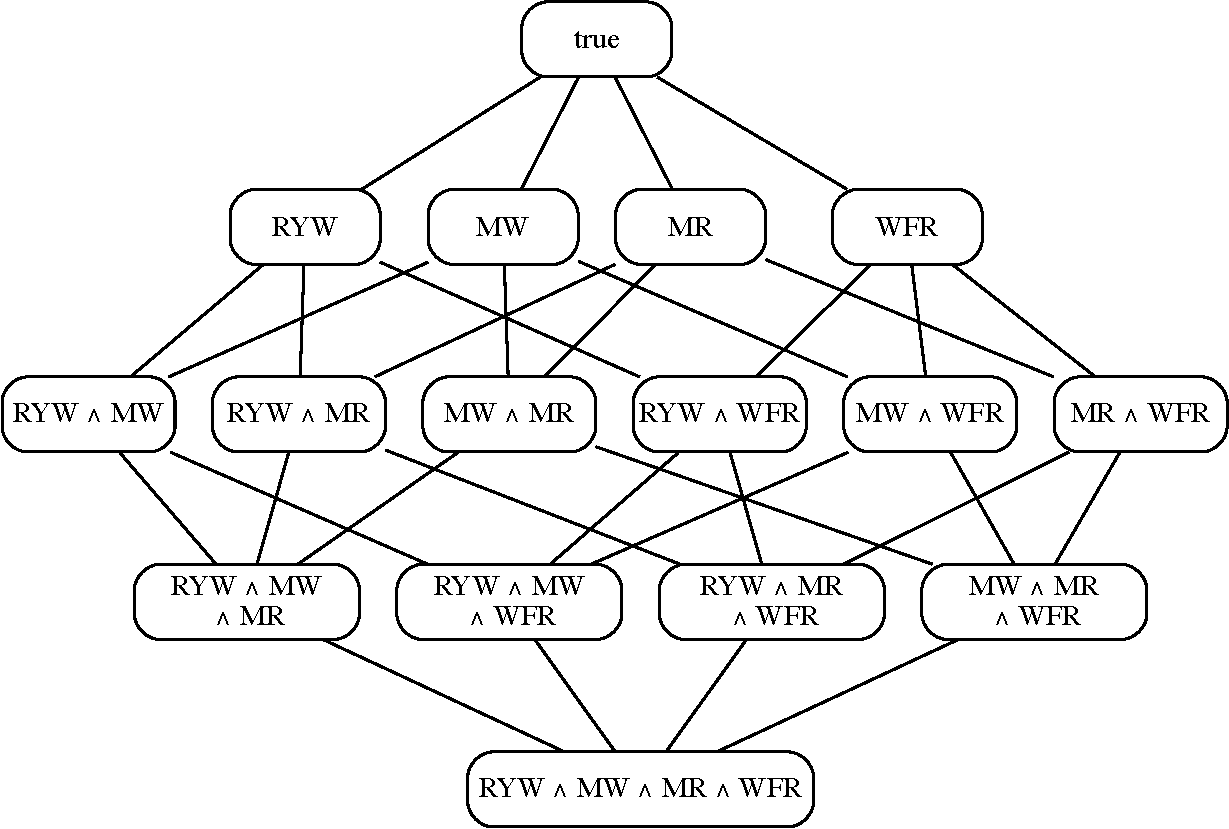
\includegraphics[width=\columnwidth]{Figures/lattice}
\end{center}
\caption{Lattice of consistency levels under session guarantees.}
\label{fig:lattice}
\end{figure}

In this scheme, the consistency level of an operation is any combination of the
above guarantees, which form a partially ordered consistency lattice show in
Figure~\ref{fig:lattice}. Each element in this lattice corresponds to a
store-consistency level, and is represented by its contract. An edge from an
upper level element to a lower level element corresponds to weaker than
relation between their corresponding contracts. Classifying a contract under
this scheme is a directed search in the lattice, starting from the bottom, and
determining the weakest consistency level under which the contract can be
satisfied. Under this scheme, \rcf{deposit} operations does not need any
guarantees, \rcf{getBalance} needs RYW and WFR ($\Delta \vdash \R{RYW} \wedge
\R{WFR} \Rightarrow \cv_{gb}$), and \rcf{withdraw} cannot be satisfied ($\Delta
\vdash \R{RYW} \wedge \R{MW} \wedge \R{MR} \wedge \R{WFR} \not\Rightarrow
\cv_{w}$).

\subsection{Soundness of Contract Classification}

We now present a meta-theoretic result that certifies the soundness of
classification-based contract enforcement. To help us state the result, we
define an operational semantics of the system described informally in
\S~\ref{sec:sysmod}:

\begin{smathpar}
\renewcommand{\arraystretch}{1.2}
\begin{array}{lclcl}
{\it op} 	& \in & \mathtt{Operation} \\
{\tau}		& \in & \mathtt{Consistency Class} 	& \coloneqq & {\sf ec},{\sf cc},{\sf sc} \\
{\sigma} 	& \in & \mathtt{Session} 					 	& \coloneqq & \cdot \ALT \langle op,\tau \rangle; \sigma \\
\Sigma 		& \in & \mathtt{Session\;Soup}   	 	& \coloneqq & \sigma \pll \Sigma \ALT \emptyset \\
					&			&	\mathtt{Config}		  			 	& \coloneqq & \E,\Sigma \\
\end{array}
\end{smathpar}

We model the system as a tuple $\E,\Sigma$, where the axiomatic execution $\E$
captures the data store's current state, and session soup $\Sigma$ is the set
of concurrent client sessions interacting with the store. A session $\sigma$ is
a sequence of pairs composed of replicated data type operations $\mathit{op}$,
tagged with the consistency class $\tau$ of their contracts (as determined by
the contract classification scheme). We assume a reduction relation of form:

\begin{smathpar}
  \auxred{} {\E,\langle op,\tau \rangle;\sigma \pll \Sigma} {\eff}
    {\E',\sigma \pll \Sigma}
\end{smathpar}

\noindent on the system state. The relation captures the progress of the
execution (from $\E$ to $\E'$)  due to the successful completion of a client
operation $\mathit{op}$ from one of the sessions in $\Sigma$, generating a new
effect $\eff$. If the resultant execution $\E'$ satisfies the store contract
$\cv_\tau$ (i.e., $\E \models \cv_\tau$), then we say that the store has
\emph{enforced} the contract $\cv_\tau$ in the execution $\E'$. With help of
the operational semantics, we now state the soundness of contract enforcement
as follows:

\begin{theorem}[Soundness of Contract Enforcement]
\label{thm:classification-sound}
Let $\cv$ be a well-formed contract of a replicated data type operation
$\mathit{op}$, and let $\tau$ denote the consistency class of $\cv$ as
determined by the contract classification scheme. For all well-formed execution
states $\E$, $\E'$ such that
$\auxred{} {\E,\langle op,\tau \rangle;\sigma \pll \Sigma} {\eff} {\E', \sigma
\pll \Sigma}$, if $\E' \models \cv_\tau[\eff/\cureff]$, then $\E' \models
\cv[\eff/\cureff]$
\end{theorem}

\noindent The theorem states that if a data store correctly enforces $\scc$,
$\ccc$, and $\ecc$ contracts in all well-formed executions, then the same
store, extended with the classification scheme shown in
Figure~\ref{sem:classify}, can enforce all well-formed \name contracts. The
proof of the theorem is given below:

\begin{proof}
  Hypothesis:
  \begin{smathpar}
  \begin{array}{cr}
    \auxred{} {\E,\langle op,\tau \rangle;\sigma \pll \Sigma} {\eff}
    {\E', \sigma \pll \Sigma} & H\npp\\
    \E' \models \cv_\tau[\eff/\cureff] & H\npp\\
  \end{array}
  \end{smathpar}
  Since $\tau$ is the contract class of $\cv$, by inversion, we have
  $\cv \le \cv_\tau$. By the definition of $\le$ relation:
  \begin{smathpar}
  \begin{array}{cr}
    \Delta \vdash \forall \cureff. \cv_\tau \Rightarrow \cv & H\npp\\
  \end{array}
  \end{smathpar}
   Since $\eff$ denotes new effect, it is a fresh variable that does
   not occur free in $\Delta$. From $H3$, after instantiating bound
   $\cureff$ with $\eff$, we have:
  \begin{smathpar}
  \begin{array}{cr}
    \Delta \vdash \cv_\tau[\eff/\cureff] \Rightarrow \cv[\eff/\cureff]
      & H\npp\\
  \end{array}
  \end{smathpar}
  Due to the soundness of natural deduction for first-order logic,
  $H4$ implies that for all models $\mathcal{M}$ such that
  $\mathcal{M} \models \Delta$, if $\mathcal{M} \models
  \cv_\tau[\eff/\cureff]$ then $\mathcal{M} \models
  \cv[\eff/\cureff]$. Since $\E'$ is well-formed, we have:
  \begin{smathpar}
  \begin{array}{cr}
    \E' \models \Delta & H\npp\\
  \end{array}
  \end{smathpar}
  Proof follows from $H1$, $H4$, and $H3$.
  \hfill \qed
\end{proof}

It is important to note that Theorem~\ref{thm:classification-sound}
does not ascribe any semantics to the reduction relation
($\xrightarrow{}$). As such, it makes no assumptions about how the
store actually implements ${\sf ec}$, ${\sf cc}$ and ${\sf sc}$
guarantees. The specific implementation strategy is determined by the
operational semantics of the store, which \emph{defines} the reduction
relation for that particular store. The following section describes
operational semantics of the store used by the \name implementation.
